%
% Introduction
%

\chapterimage{Galileos-telescope-002.pdf} % Chapter heading image

\chapter{Introduction}
\label{chap:Introduction}

\begin{quote}
\begin{flushright}
\emph{If presented with a choice between indifferent alternatives,\\
then one ought to select the simplest one.}\\
Occam's razor principle 
\end{flushright}
\end{quote}
\bigskip

We find ourselves in an age where knowledge has become one of our most valued resources, driving both economic progress and societal well-being. Science continually provides us with deeper insights and practical solutions, shaping our daily lives through innovations ranging from advanced medical therapies to transformative digital technologies. However, the path of scientific exploration is neither straightforward nor free from significant barriers. Despite remarkable progress, our current scientific methodologies remain bounded by inherent limitations that restrict our ability to fully understand and address complex issues.

These limitations manifest in various ways, including fragmented research efforts, rigid disciplinary boundaries, and an often narrow approach to funding allocation, which tends to overlook bold, high-risk projects with transformative potential. Moreover, the conventional metrics of scientific success frequently incentivize incremental progress rather than genuinely groundbreaking discoveries, limiting innovation's pace and scope.

The theory of nescience emerges from the critical recognition of these challenges and the profound need to overcome them. It advocates a renewed approach to exploring the unknown, driven by curiosity and the willingness to question accepted knowledge rigorously. By systematically addressing the limitations inherent in contemporary scientific practice, our objective is to provide robust frameworks that significantly enhance our capability to solve real-world problems and catalyze meaningful advancements across diverse fields.

%
% Section: Entities
%

\section{Scientific Knowledge}

The pursuit of knowledge begins with identifying the \emph{entities} we seek to understand, entities that are often extraordinarily diverse. Mathematicians focus on abstract concepts, biologists on living organisms, and engineers on machines. Our quest for understanding is fundamentally driven by our need to predict outcomes, solve problems, and navigate the complexities of the world around us. For instance, we know that applying sufficient heat to wood will ignite a fire, or that a fever may indicate a viral infection. Practical problem-solving, therefore, hinges crucially on our ability to recognize patterns and create simplified models of these entities. These models empower us to interact beneficially with the world.

Yet, while ideally, we strive to build precise \emph{descriptions} capable of fully reconstructing the entities we study, in reality, such perfection often eludes us, particularly with abstract entities. Consequently, we rely on \emph{representations}, texts or datasets capturing essential details of these entities. Physicists might represent an entity through experimental results; computer scientists through measured data; sociologists through observed facts. Figure \ref{fig:representationProblem} illustrates this critical interplay: although we aim to directly describe entities, practically, our descriptions are based on constructed representations.

% A4
% \begin{figure}[t]
% \centering
% \begin{tikzpicture}
%     \node[draw, ellipse, minimum width=3cm] (entities) at (0,0) {Entities};
%     \node[draw, ellipse, minimum width=3cm] (representations) at (5,0) {Representations};
%     \node[draw, ellipse, minimum width=3cm] (descriptions) at (10,0) {Descriptions};
% 
%     \draw[-{Latex[length=3mm]}] (representations) -- node[above,midway] {encode} (entities);
%     \draw[-{Latex[length=3mm]}] (descriptions) -- node[above,midway] {model} (representations);
%     \draw[dashed,-{Latex[length=3mm]}] (descriptions) to [bend right=45] node[above,midway] {explain?} (entities);
% \end{tikzpicture}
% \caption{\label{fig:representationProblem}The Problem of Understanding}
% \end{figure}

% Octavo
\begin{figure}[t]
\centering
\begin{tikzpicture}
    \node[draw, ellipse, minimum width=1.5cm] (entities) at (0,0) {Entities};
    \node[draw, ellipse, minimum width=1.5cm] (representations) at (4.25,0) {Representations};
    \node[draw, ellipse, minimum width=1.5cm] (descriptions) at (9,0) {Descriptions};

    \draw[-{Latex[length=3mm]}] (representations) -- node[above,midway] {encode} (entities);
    \draw[-{Latex[length=3mm]}] (descriptions) -- node[above,midway] {model} (representations);
    \draw[dashed,-{Latex[length=3mm]}] (descriptions) to [bend right=45] node[above,midway] {explain?} (entities);
\end{tikzpicture}
\caption{\label{fig:representationProblem}The Problem of Understanding}
\end{figure}

Understanding the effectiveness of our descriptions involves examining potential errors deeply. Firstly, encoding methods can introduce errors, what we call \emph{miscoding}\index{Miscoding}. Secondly, our descriptions themselves may fail to precisely recreate the encoded representations, resulting in \emph{inaccuracy}\index{Inaccuracy}. Lastly, due to human cognitive limitations, descriptions should not become unnecessarily complex, introducing \emph{surfeit}\index{Surfeit}.

Collectively, miscoding, inaccuracy, and surfeit hinder our quest for clear understanding and reliable predictions. By amalgamating these three error types into a single measure, known as \emph{nescience}\index{Nescience}, we quantify our lack of knowledge, providing an essential tool for systematically addressing and reducing our ignorance.

%
% Section: Entities
%

\section{Entities}

At the core of our theory of nescience is the recognition that science is, at its essence, a quest to understand the world around us. Throughout history, scientists have examined an extraordinary variety of things (planets, particles, languages, ecosystems, human societies, and much more) in an effort to uncover patterns, formulate explanations, and make predictions. These things we seek to understand, which we refer to as \emph{entities}\index{Entity}, form the basis of all scientific activity. An entity might be a tangible object, such as a chemical compound or a cell, or something more abstract, like a mathematical function or a cultural practice.

The scope of what science might investigate is vast and continually evolving. New technologies, shifting societal needs, and fresh philosophical insights regularly bring new entities into view. What unifies this effort is a foundational belief: that some of these entities can be understood through science. That is, we hold that at least part of the unknown is ultimately knowable (see Section \ref{sec:what-is-an-entity}). This belief fuels the scientific drive to bring clarity to what was once obscure, to shed light on complexity, and to convert speculation into knowledge. Understanding how we fall short of this ideal, how ignorance persists and why, is the starting point for the theory of nescience.

One important conceptual difficulty we face is that the set of all entities under consideration, what we refer to symbolically as $\mathcal{E}$, cannot be rigorously defined in mathematical terms, except to say that it must be non-empty. This may seem like a minor point, but it carries deep implications.

In mathematics, the idea of a "set of everything" is fraught with contradictions. For instance, if we tried to construct a set that included absolutely all things (physical objects, abstract ideas, ...) we would quickly encounter logical problems. This is why we deliberately avoid the notion of a universal set in the theory of nescience. A key reason for this caution lies in Cantor's theorem\index{Cantor's theorem}, which we discuss further in Section \ref{sec:descriptions_entities}. Cantor's result shows that for any set, the collection of all its subsets is strictly larger in size than the set itself. As a consequence, it becomes impossible to form a set that includes everything without running into contradictions. Similarly, we steer clear of problematic constructions that lead to paradoxes, such as Russell's paradox\index{Russell's paradox}, another example covered in Section \ref{sec:descriptions_entities}, which illustrates how self-referential sets can collapse logical consistency.

These mathematical constraints are not mere formalities; they serve a vital purpose. By enforcing clear boundaries around the sets of entities we analyze, we ensure that the theory we are building remains coherent, consistent, and applicable. It allows us to focus our attention on meaningful, well-defined domains where real progress in understanding can be made.

In practice, we will work with well-defined sets, each associated with a specific domain of inquiry and its unique goals. These sets provide a practical framework for applying our theory to real-world contexts. For example, in mathematics, such a set might include different classes of abstract structures such as groups, functions, or topological spaces. In biology, it could encompass the vast diversity of living organisms, from microscopic bacteria to complex multicellular animals. In the realm of social sciences, the entities might include human behaviors, social systems, or economic models. And in computer science, we may focus on algorithms, data structures, and executable programs.

By tailoring our analysis to these different sets, we are able to apply a unified theoretical framework to a wide variety of disciplines. This adaptability is one of the strengths of our approach: it allows us to measure and reduce human ignorance, or nescience, in fields with very different kinds of entities. Our goal is not only to improve our theoretical understanding of these domains but also to contribute practical tools that can support deeper insights, better decision-making, and more effective problem-solving across the sciences and beyond.

%
% Section: Representations
%

\section{Representations}

\begin{figure}[t]
\centering

\begin{tikzpicture}
  % Oval 1
  \node[draw, ellipse, minimum width=3cm, minimum height=6cm, label=below left:{$\mathcal{E}$}] (oval1) at (-2,0) {};

  % Oval 2
  \node[draw, fill=gray!20, ellipse, minimum width=2cm, minimum height=3cm] (oval2) at (-2,1) {};

  % Small circles inside Oval 2
  \node[draw, fill=black, circle, inner sep=0.05cm, label=below:{$e_1$}] (circle1) at (-2, 1.5) {};
  \node[draw, fill=black, circle, inner sep=0.05cm, label=below:{$e_2$}] (circle2) at (-2, 0.5) {};

  % Small circle inside Oval 1
  \node[draw, fill=black, circle, inner sep=0.05cm, label=below:{$e_3$}] (circle3) at (-2,-1) {};

  % Question mark inside Oval 1
  \node[draw, fill=black, circle, inner sep=0.05cm, label=below:{?}] (question) at (-2,-2) {};

  % Vertical Line
  \draw[thick] (0,-3) -- (0,3);
  \node at (0,-3.5) {oracle};

  % Oval 4
  \node[draw, fill=gray!20, ellipse, minimum width=2cm, minimum height=4cm, label=above right:{$\mathcal{R}_{\mathcal{E}}$}] (oval4) at (2,1) {};

  % Small circles inside Oval 4
  \node[draw, fill=black, circle, inner sep=0.05cm, label=below:{$r_1$}] (circle5) at (2,1.5) {};
  \node[draw, fill=black, circle, inner sep=0.05cm, label=below:{$r_2$}] (circle6) at (2,0.5) {};

  % Oval 3
  \node[draw, ellipse, minimum width=2cm, minimum height=4cm, label=below right:{$\hat{\mathcal{R}}_\mathcal{E}$}] (oval3) at (2,-1) {};

  % Small circle inside Oval 3
  \node[draw, fill=black, circle, inner sep=0.05cm, label=below:{$r_3$}] (circle4) at (2,-2) {};

  % Curved arrows
  \draw[->] (circle5) to[bend right=40] (circle1);
  \draw[->] (circle6) to[bend right=40] (circle2);
  \draw[->] (circle4) to[bend left=40] (question);
\end{tikzpicture}

\caption{\label{fig:entities_topics}Entities and Representations.}
\end{figure}

In many instances, entities cannot be directly scrutinized through scientific analysis, particularly if they are abstract. As a result, we are compelled to rely on representations, i.e., symbolic encodings that stand in for the entities we aim to understand. We designate the collection of strings that encode the entities of $\mathcal{E}$ as $\mathcal{R_\mathcal{E}}$. These strings, referred to as \emph{representations}\index{Representation}, may differ depending on the application of the theory of nescience. In certain scenarios, entities may inherently be string-based (e.g., computer programs), while others might be abstract objects that require encoding into string format (e.g., human needs). It is not uncommon for a single entity $e \in \mathcal{E}$ to have multiple valid representations within $\mathcal{R_\mathcal{E}}$, for example, a text-based description, a diagram saved as a computer file, or a collection of empirical measurements. Each representation emphasizes different aspects of the entity and may be better suited to particular investigative goals or scientific approaches. Transforming abstract entities into symbol strings in a manner that faithfully captures their complexities and subtleties remains a formidable and unresolved challenge. Consequently, the exact composition of $\mathcal{R_\mathcal{E}}$ often eludes us.

In a world where understanding depends on symbolic surrogates, the idea of constructing an encoding function $f:\mathcal{E} \rightarrow \mathcal{R_\mathcal{E}}$ becomes not only attractive but essential. The function $f$ represents an idealized encoding process: it assigns to each entity $e \in \mathcal{E}$ one of its symbolic representations $r \in \mathcal{R_\mathcal{E}}$. In essence, this function models the act of transforming something we wish to understand (like a physical object, a biological system, or an abstract concept) into a format that can be studied, manipulated, or stored using symbols, typically as strings. In practice, such a function would allow us to systematically move from the domain of real-world or conceptual entities to their formal encodings, which are necessary for analysis in science, computation, and communication. However, defining such a function is no trivial task, precisely because $\mathcal{E}$ itself is not well defined. The boundaries of what should or should not be included in $\mathcal{E}$ are inherently blurred. For example, we still lack a precise and universally accepted definition of what constitutes a human need.

To grapple with this indeterminacy, one may resort to theoretical constructs such as the \emph{oracle Turing machine}\index{Oracle Turing machine} (see Chapter \ref{chap:Computability}). While a standard \emph{Turing machine}\index{Turing machine} serves as a mathematical model of computation, the oracle variant introduces a conceptual leap: it simulates a computer with access to an external source of information. The oracle Turing machine can be imagined as a theoretical computer connected not to the actual internet of today, but to an idealized version, an omniscient information source containing perfect knowledge about everything that exists or could exist. This imaginary machine is allowed to submit string-based queries to this vast external database. For instance, it might ask whether a given string $r$ encodes any entity in $\mathcal{E}$. Unfortunately, formulating the question “does $r$ represent $e$?” would require expressing $e$ itself as a string of symbols. And since we do not know how to encode $e$ in advance, we cannot construct such a query. This irony captures the very dilemma we aim to address, the tension between what can be queried, what can be known, and the inherent limitations of representation in scientific inquiry.

From a practical perspective, we typically approximate the set $\mathcal{R}_\mathcal{E}$ with another set $\hat{\mathcal{R}}_\mathcal{E}$ of strings, which we consider to be adequate representations of the entities of $\mathcal{E}$. In scientific practice, these representations have traditionally taken the form of illustrations or images (e.g., in biology), collections of factual data (e.g., in sociology), or experimental results (e.g., in physics). With recent significant advancements in the capability of computers to gather and store data, a novel and potent method for encoding entities has emerged: using vast data sets as representations. It's essential to note that in the encoding process, our objective is not to find the shortest possible representation of the entities but to seek out high-quality representations.

It's crucial to acknowledge that in numerous practical scenarios, the chosen representations of abstract entities may not fully encapsulate all nuances of the original objects. This means we are grappling with simplified abstractions of reality, which could potentially curtail our capacity to make sweeping assertions about nature (see Chapter \ref{chap:Miscoding}).

\begin{example}
\label{ex:animals_DNA}
If we're studying animals (the set $\mathcal{E}$), we could use a binary encoding of their DNA (the set $\mathcal{R_\mathcal{E}}$) as representations. While our current technology doesn't allow us to bring a creature to life solely from its DNA, theoretically, it could be feasible. However, DNA alone doesn't fully replicate the original animal, as it doesn't include life experiences. For instance, how would we represent a cat that only has three legs due to an accident? That detail is not recorded in its DNA. If our goal is to study the traits of certain species, working with the DNA of a representative sample of individuals within each species would be adequate. However, if we're studying specific individuals within a species, we would also need a way to encode each animal's history or the details not encapsulated by the DNA.
\end{example}

Working with strings as representations (the set $\mathcal{R}_\mathcal{E}$) inevitably results in certain entities lacking any corresponding encoding (see the gray areas in Figure \ref{fig:entities_topics}; specifically, entity $e_3$ has no representation). This limitation becomes particularly evident when the set of entities is uncountable. For example, if $\mathcal{E}$ is the set of real numbers, many elements cannot be represented, since we restrict representations to finite binary strings. Real numbers that require infinite precision (such as most irrational numbers) cannot be fully encoded. This mismatch reveals a deeper asymmetry: in many domains of knowledge, the space of conceivable problems or entities far exceeds the space of valid, encodable representations. Intuitively, this suggests that in such domains, the quantity of problems may exceed the number of solutions.

Using approximations of representations (the set $\hat{\mathcal{R}}_\mathcal{E}$) can also result in some representations encoding the wrong entities, as illustrated by representation $r_3$ in Figure \ref{fig:entities_topics}. This occurs because our knowledge about the entities in $\mathcal{E}$ is often incomplete or imprecise, which can lead us to construct representations that appear valid but fail to correspond to the intended entity.

Another issue with incomplete knowledge is the possibility of having unknown entities whose existence we are unaware of. For instance, representation $r_1$ in Figure \ref{fig:entities_topics} is not part of the set $\hat{\mathcal{R}}_\mathcal{E}$ and is therefore overlooked by researchers despite being the representation of a knowable entity $e_1$. One of the objectives of this book is to provide a procedure to uncover new, previously unknown, research entities from the set $\mathcal{R}_\mathcal{E}$ (refer to Section \ref{sec:intro_research_topics} and Chapter \ref{chap:computational-creativity}).

%
% Section: Descriptions
%

\section{Descriptions}

Upon identifying the set $\mathcal{R}$ of potential representations, we are faced with the deeper motivation that drives much of scientific inquiry: the desire to bring order to the complexity of the world. To do this, we must devise appropriate methods to describe these representations, an endeavor that underlies our attempt to form theories or models that articulate how the world operates. Our limited cognitive capacities as humans compel us to work with simplified, yet insightful, models of nature. These abstractions help us interpret phenomena and forecast the consequences of our actions. Descriptions also change over time, as our understanding of the entities studied improves.

\begin{example}
To anchor these ideas in the concrete, consider the evolving effort to describe the macroscopic behavior of the physical universe (the entity $e$). The sequence of proposed descriptions includes Aristotelian physics, Cartesian mechanics, Newtonian laws, Einstein's relativity, and, potentially, superstring theory. Each successive model attempts to refine our grasp of reality. Among these, Einstein's theory currently stands as the most complete, given that alternatives like superstring theory still await experimental corroboration.
\end{example}

Defining a valid description for an entity is not merely a technical challenge; it embodies a fundamental limitation of knowledge. The Berry paradox\index{Berry paradox} serves as a compelling reminder of these philosophical intricacies. A phrase like "the smallest positive integer not definable in less than twelve words" becomes paradoxical by succeeding in doing just that within eleven words. To avoid such pitfalls, the theory of nescience imposes stricter demands: a valid description must be a finite symbol string that allows us to effectively and completely reconstruct a possible representation of the original entity. By "effectively," we mean that this reconstruction can be performed by a machine, or computer, without human intervention.

From Newton's formulation of classical mechanics to today's explorations, the scientific journey has been shaped by the pursuit of mathematical models. The theory of nescience follows this lineage but extends it by demanding that models be computable, i.e. executable by computers. This requirement of computability of descriptions allows us to remove many of the paradoxes traditionally associated with the concept of description. In this light, science becomes not only a quest for understanding but also a computable-driven endeavor to approximate reality.

Descriptions\index{Description} are typically divided into two components: a Turing machine\index{Turing machine} $TM$ (a computer program) that encapsulates all the regularities found in the entity's representation (the compressible part), and an input string $a$ that contains a literal description of the remaining elements (the non-compressible part). This dualistic nature of descriptions parallels traditional distinctions in science, such as theories and assumptions, theories and initial conditions, problems and specific problem instances, species and individuals, and so on. For instance, a description might consist of a system-modeling set of differential equations (the compressible part), accompanied by a compilation of initial conditions (the non-compressible part). The precise interpretation of the pair $TM, a$ relies on the specific characteristics of the entity set to which the theory is applied.

\begin{figure}[t]
\centering
\begin{tikzpicture}

    % Draw ovals
    \node[draw,ellipse,minimum width=2.2cm,minimum height=3cm] (entityOval) at (0,0) {};
    \node[draw,ellipse,minimum width=2.2cm,minimum height=3cm] (representationOval) at (3.5,0) {};
    \node[draw,ellipse,minimum width=2.2cm,minimum height=3cm] (descriptionOval) at (7,0) {};
    
    % Draw circle nodes
    \node[fill=black,circle,label={[font=\footnotesize]below:Entity}] (entity) at (entityOval) {};
    \node[fill=black,circle,label={[font=\footnotesize]below:Representation}] (representation) at (representationOval) {};
    \node[fill=black,circle,label={[font=\footnotesize]below:Description}] (description) at (descriptionOval) {};
    
    % Draw arrows
    \draw[-{Latex[length=3mm]},>=stealth,thick,bend right] (representation.north) to node[above]{encode} (entity.north);
    \draw[-{Latex[length=3mm]},>=stealth,thick,bend right] (description.north) to node[above]{model} (representation.north);

\end{tikzpicture}
\caption{\label{fig:entities_topics_models}Entities, representations and descriptions.}
\end{figure}

Figure \ref{fig:entities_topics_models} illustrates the relationship between entities, representations, and descriptions. The set of all potential descriptions is denoted by $\mathcal{D}$. However, not all strings qualify as valid descriptions: each must be grounded in a Turing machine, ensuring that it is computationally meaningful. Furthermore, not every valid description corresponds to a legitimate representation. Since representations $r$ can be described in multiple ways, the overarching scientific goal emerges as the search for the shortest possible description $d$ that faithfully reconstructs the observed data.

However, a fundamental obstacle lies in the incomputability of this task. As discussed in Chapter \ref{chap:Algorithmic_Information}, there exists no general procedure to determine the shortest program that outputs a given string. This impossibility extends to representations, rendering the pursuit of optimal scientific models as a challenge beyond computer capabilities. As a result, science must rely on heuristic strategies to approximate ideal solutions. Collectively, these heuristics define what we call the \emph{scientific method}\index{Scientific method}.

The theory of nescience is driven by the desire to understand, and ultimately quantify, the various errors that arise in the process of scientific discovery. Figure \ref{fig:entities_topics_models} provides the conceptual framework for this endeavor. In Sections \ref{sec:ch1_miscoding}, \ref{sec:introduction:inaccuracy}, and \ref{sec:ch1_surfeit}, we introduce metrics designed to capture distinct sources of error. These components are then synthesized in Section \ref{sec:ch1_nescience} into a single, unified measure: nescience. Although inherently uncomputable, this measure formally expresses the extent to which a given research entity remains poorly understood. It highlights not only the boundaries of current knowledge but also the areas most deserving of scientific attention.

%
% Section: Miscoding
%

\section{Miscoding}
\label{sec:ch1_miscoding}

As we've observed, in many scientific disciplines, the effort to understand the world often begins with an elusive challenge: the entities we wish to study, denoted as the set $\mathcal{E}$, do not always lend themselves to clear or complete representations. Some of these entities are too abstract, others too complex, and many remain partially known. This mismatch between the reality we wish to grasp and the means we have to represent it is not merely a technical limitation, it reflects the very heart of scientific inquiry.

The scientist's journey, then, often starts in uncertainty. We make do with approximations, crafting descriptions that we hope capture enough truth to be useful. Yet, we are aware that these representations carry errors. Our goal becomes not just to encode entities, but to quantify the error introduced by using these inaccurate representations.

\begin{figure}[t]
\centering
\begin{tikzpicture}
  % Oval 1
  \node[draw, ellipse, minimum width=3cm, minimum height=4cm, label=below left:{$\mathcal{E}$}] (oval1) at (-2,0) {};

  % Small circles inside Oval 1
  \node[draw, fill=black, circle, inner sep=0.05cm, label=below:{e}] (circle1) at (-2, 1) {};
  \node[draw, fill=black, circle, inner sep=0.05cm, label=below:{?}] (circle2) at (-2, 0) {};

  % Vertical Line
  \draw[thick] (0,-2.5) -- (0,2.5);
  \node at (0,-3) {oracle};

  % Oval 2
  \node[draw, fill=gray!20, ellipse, minimum width=1.25cm, minimum height=1cm, label=right:{$\mathcal{R}_{e}$}] (oval2) at (2,1.05) {};

  % Small circles inside Oval 2
  \node[draw, fill=black, circle, inner sep=0.05cm, label=below:{$r$}] (circle3) at (2,1) {};

  % Oval 3
  \node[draw, ellipse, minimum width=3cm, minimum height=4cm, label=below right:{$\mathcal{R}$}] (oval3) at (2,0) {};

  % Small circle inside Oval 3
  \node[draw, fill=black, circle, inner sep=0.05cm, label=below:{$r'$}] (circle4) at (2,0) {};

  % Curved arrows
  \draw[->] (circle3) to[bend right=40] (circle1);
  \draw[->] (circle4) to[bend right=40] (circle2);
\end{tikzpicture}
\caption{\label{fig:miscoding}Miscoding of topics.}
\end{figure}

We propose to measure the \emph{miscoding}\index{Miscoding} of an inaccurate representation $r'$ by assessing how difficult it is to transform this flawed representation into a correct one. In more technical terms, this difficulty is expressed as the length of the shortest computer program that, when given $r'$ as input, is able to produce the accurate representation $r$. Figure \ref{fig:miscoding} provides a visual depiction of this process. The set $\mathcal{R}_e$ consists of all the strings that are considered accurate representations of the entity $e$. If  falls outside this set, it means our understanding is flawed. Miscoding represents the cost of bridging that gap. Importantly, this cost is not about computational time or speed. It is about descriptional complexity, how much must be said, or programmed, to repair the mistakes. If $r'$ contains inaccuracies, the required program must identify these deviations and correct them. If instead $r'$ lacks key information altogether, the missing content must be embedded within the program itself. In this way, miscoding becomes a reflection of our ignorance: the larger the program needed, the more knowledge we have to include to arrive at the truth. Miscoding measures how much we still need to learn before our representations truly encode the entities we seek to understand.

However, the previous method of measuring miscoding does not fully capture our intuitive understanding of what it means for a representation to be flawed. There is a deeper issue that emerges when a representation includes more than what is necessary. In other words, it may not only be inaccurate by omission but also by addition. Consider a situation where the representation $r'$ contains extra information that is irrelevant or unrelated to the entity $e$ we are trying to understand. This surplus information is not just noise, it actively distorts the description by forcing any model based on $e$ to account for elements that have no bearing on the actual entity. The result is a bloated and misleading representation. The description becomes longer not because the entity itself is more complex, but because our flawed representation includes unnecessary baggage. This problem is not just theoretical. In real-world scientific practice, we frequently encounter such scenarios. Imagine an experiment where multiple variables are being recorded, but only a few of them actually influence the outcome. If we do not yet know which variables are relevant, our current models might treat all recorded features as potentially significant. This lack of understanding can lead us to build explanations and predictors around elements that are, in reality, unrelated to the entity or phenomenon of interest.

To account for this kind of misrepresentation, we must expand our definition of miscoding. We need to ask not only how much effort is required to fix an inaccurate representation, but also how much effort it would take to reconstruct that flawed version from the correct one $r$. The higher this effort, the worse the representation is, as it suggests that the inaccurate description deviates significantly from what is accurate. This leads us to introduce the a second measure, as the length of the shortest computer program that can output the incorrect description $r'$ given the accurate one $r$. Only by considering both directions, how difficult it is to go from $r'$ to $r$, and how difficult it is to go from $r$ to $r'$, can we fully assess the degree of miscoding. We therefore define miscoding as the maximum of these two values. This revised definition acknowledges that misinformation can come in multiple forms. It captures both the missing and the misleading, recognizing that a poor representation might not only fail to say what is necessary, but might also say unnecessary things. In this way, miscoding becomes a more complete reflection of the divergence between what we currently believe and what truly is.

Nevertheless, this latest definition still poses practical challenges. In many cases, the same entity can be described in multiple, equally valid ways. This multiplicity creates a dilemma: what should we do when our inaccurate representation $r'$ is far from one correct representation $r_1$, but quite close to another valid one $r_2$? Judging  solely by its distance to $r_1$ could unfairly suggest a high level of miscoding, when in fact $r_2$ may be a legitimate approximation of $e$.

The core issue here is that correctness is not always unique. Scientific and mathematical entities often admit many forms of expression—each highlighting different properties, or suited for different contexts. Penalizing a representation for not being similar to just one of these correct forms would ignore the richness and flexibility of representation.

\begin{example}
\label{ex:leibnez-wallis}
Consider $e$ as the abstract entity known as the "Pi constant", the ratio of a circle's circumference to its diameter. Let $r$ be the Wallis product\index{Wallis' product}, expressed as $2 (\frac{2}{1} \cdot \frac{2}{3} \cdot \frac{4}{3} \cdot \frac{4}{5} \cdot \frac{6}{5} \cdot \ldots)$, a well-known infinite product that converges to $\pi$. Suppose $r'$ is the infinite series $4 (1 - \frac{1}{3} + \frac{1}{5} - \frac{1}{7} + \ldots)$ which corresponds to the Leibniz series\index{Leibniz's series}. Although $r'$ is structurally very different from $r$, it also accurately represents the same entity $e$. To declare $r'$ as highly miscoded with respect to $r$ would be misleading, because $r'$ is not an error, it's an alternative, equally correct expression.
\end{example}

As example \ref{ex:leibnez-wallis} indicates, defining miscoding poses challenges because the set $\mathcal{R}_e$ of valid representations for the entity $e$ is generally unknown. Theoretically, we could rely again on the oracle Turing machine\index{Oracle Turing machine} to solve this problem. However, as observed, we can't ask the oracle if the string $r$ is a valid representation of our interested entity $e$ (the set $\mathcal{R}_e$), since that would require us to provide a valid encoding of $e$ as a string of symbols, which typically can't be done. Perhaps, all we can do is ask this oracle how close a given string $r$ is to being a valid description of some entity in the entire set of entities $\mathcal{R}_\mathcal{E}$.

With this constraint in mind, we have to define the miscoding of a representation as the smallest possible discrepancy, as judged by the oracle, between our given string and any valid representation of any entity. In this way, we allow the oracle to search through the universe of all correct representations, looking for the one that is most similar to our candidate. This definition enables us to talk about miscoding even in the absence of a known ground truth. 

But there is one final complication we must confront. Because this definition of miscoding does not rely on knowing the actual entity being represented, it opens the door to a subtle yet critical problem: we might not be representing what we think we are. In other words, our descriptions might be well-formed and internally consistent, yet point to an entirely different entity than we had intended. This kind of mistaken identity is not just a philosophical curiosity, it has occurred repeatedly in the history of science. Researchers have often believed they were investigating one phenomenon, only to later discover that their results pertained to something entirely different.

\begin{example}
In the late eighteenth century, chemist Joseph Priestley believed he was studying a substance called "phlogiston"\index{Phlogiston}, which was thought to be a fire-like element released during combustion. All of his experiments and representations were constructed around this idea. However, in reality, Priestley was observing the properties of a completely different entity: oxygen. Though his descriptions were coherent and reproducible, they were ultimately anchored to the wrong conceptual foundation.
\end{example}

According to the theory of nescience, our role as researchers goes beyond the mere identification of correct representations for the entities we wish to understand. It also involves a deeper and more ambitious task: uncovering the principles by which an idealized oracle machine would reconstruct the original entities given their representations. In other words, it is not enough to arrive at accurate representations, we must also strive to understand why these representations are accurate, what makes them effective, and how they reflect the intrinsic structure of the underlying entities, by understanding how this hypothetical abstract oracle would work. This shift in perspective moves us from a practice of isolated trial and error to a more reflective inquiry into the nature of scientific representation itself. Our goal is not just to find a representation that works, but to understand the encoding process more deeply.

%
% Section: Inaccuracy
%

\section{Inaccuracy}
\label{sec:introduction:inaccuracy}

In the preceding section, we explored how ignorance may arise when the representation $r'$ we use to encode an entity $e$ does not match the actual entity's correct representation $r$. That was the problem addressed by miscoding. Now, we turn to another, equally important source of ignorance, what we call \emph{inaccuracy}\index{Inaccuracy}, which emerges not from selecting the wrong representation, but from failing to describe it adequately.


In an ideal scenario, we would have a description $d$, that is, a computer program, capable of fully reconstructing the representation $r'$, even if the true representation $r$ remains unknown. However, this level of precision is rarely attainable in practice. More commonly, we rely on an approximate description $d'$, which produces a string $r''$ that resembles $r'$, but is not exactly the same. In such cases, we refer to $d'$ as an \emph{inaccurate}\index{Inaccurate description} description of the representation $r'$ (see Figure \ref{fig:inaccuracy:inaccuracy:inaccuracy}).

\begin{figure}[t]
\centering
\begin{tikzpicture}
  % Oval 1
  \node[draw, ellipse, minimum width=3cm, minimum height=4cm, label=below left:{$\mathcal{R}$}] (oval1) at (-2,0) {};

  % Small circles inside Oval 1
  \node[draw, fill=black, circle, inner sep=0.05cm, label=below:{r}] (circle1) at (-2, 1) {};
  \node[draw, fill=black, circle, inner sep=0.05cm, label=below:{r'}] (circle2) at (-2, 0) {};
  \node[draw, fill=black, circle, inner sep=0.05cm, label=below:{r''}] (circle3) at (-2, -1) {};

  % Oval 2
  \node[draw, ellipse, minimum width=3cm, minimum height=4cm, label=below right:{$\mathcal{D}$}] (oval2) at (2,0) {};

  % Small circle inside Oval 2
  \node[draw, fill=black, circle, inner sep=0.05cm, label=below:{$d$}] (circle4) at (2, 0) {};
  \node[draw, fill=black, circle, inner sep=0.05cm, label=below:{$d'$}] (circle5) at (2, -1) {};

  % Curved arrows
  \draw[->] (circle4) to[bend right=40] (circle2);
  \draw[->] (circle5) to[bend right=40] (circle3);
\end{tikzpicture}
\caption{\label{fig:inaccuracy:inaccuracy:inaccuracy}Inaccuracy of a description.}
\end{figure}

If a description is inaccurate for a representation, it is useful to have a quantitative measure of how much we deviate from accurately modeling the representation. A viable method to define this measure could be calculating the effort needed to rectify the output of our inaccurate description. In this context, the inaccuracy could be determined by the length of the shortest computer program that can generate the correct representation when fed with the incorrect one produced by the description. However, similar to the case with miscoding, to have a holistic understanding of the error associated with the description $d$, we must also calculate the difficulty of generating the inaccurate representation given the correct one. It's possible that our description $d$ models elements unrelated to the representation $r'$, and merely ignoring these elements won't solve the problem.

In other words, the inaccuracy measures how difficult it is to convert the output of the description into the intended representation, or the other way around, how difficult is to convert the representation in the output of our description. The larger the maximum of these two values, the more the description deviates from accurately capturing the intended representation.

We deliberately prefer the term \emph{inaccuracy} over the term \emph{error}. In the language of continuous systems, error includes both precision and accuracy. But in our discrete framework, where descriptions are finite symbol strings, precision loses its relevance. What matters here is how well the structure of the description aligns with the structure of the representation.

In practice, calculating the inaccuracy associated with the description of a representation is a challenging task. As previously mentioned, determining the length of the shortest computer program that can print a string is a non-computable problem. If the original entities are texts themselves, we could approximate the inaccuracy using compression algorithms. Here, the string complexity is approximated by the length of the compressed text using a compressor. If the topics are abstract entities, such as mathematical concepts, their descriptions could be derived from the result of an experiment. Hence, the inaccuracy could be based on the model's error (for instance, by calculating the length of additional information required to thoroughly describe the experiment's results given the model). In this regard, our definition of inaccuracy is a generalization of the concept of error. It can be applied to various types of entities, not only those that can be encoded as datasets.

\begin{example}
\label{ex:introduction:inaccuracy:newton}
Consider Newton's second law\index{Newton's second law} of motion, $F = ma$. Suppose we construct a dataset by applying known forces to objects of varying masses and measuring their resulting accelerations. If our goal is to study gravitational acceleration, the force and mass terms cancel, isolating acceleration as the variable of interest. Encoding this dataset in full would require a significant number of bits. Yet, recall that our objective with representations is not to minimize string length but to ensure that the encoding captures the richness and structure of the underlying phenomenon.

In this example, we draw on a historical experiment conducted by the National Bureau of Standards in Washington D.C. between May 1934 and July 1935. The dataset includes 81 measurements of acceleration in centimeters per second squared, for instance, a value like 980,078. Using a uniform 20-bit encoding per measurement, the full dataset requires 1,620 bits. Suppose a model predicts a gravitational acceleration of $980,000 cm/s^2$ plus noise. If encoding the dataset using this model only requires 453 bits, the model's inaccuracy is estimated as:
\[
\frac{453}{1,620} = 0.27
\]
This tells us how much information must be added to the model to fully account for the empirical data. It quantifies the gap between representation and reality.
\end{example}

What this example illustrates is a profound ambiguity: when our models and our data disagree, we cannot determine, in general, whether the failure lies in the experiment (miscoding) or in the model (inaccuracy). This ambiguity is not a flaw of the framework, it is a reflection of the inherent uncertainty we face when attempting to describe the world. And it is precisely this uncertainty that the theory of nescience seeks to explore, quantify, and ultimately reduce.

%
% Section: Surfeit
%

\section{Surfeit}
\label{sec:ch1_surfeit}

In our pursuit of understanding, we often encounter a paradox: the more complex and verbose our explanations, the less confident we should be in the depth of our knowledge. Complexity, when unnecessary, signals confusion. When we struggle to explain a concept concisely, it is likely because our grasp of it remains partial. This observation reveals a deeper motivation behind scientific inquiry: the drive to eliminate what is superfluous, to strip our models down to their essential structure. By doing so, we gain clarity not only in explanation but also in prediction and control.

Science depends on descriptions, most often in the form of mathematical models, to interpret the past, predict the future, trace the connections between cause and effect, and engineer solutions to practical problems. But these models, to serve us effectively, must remain within the limits of our cognitive capacities. As scientists and engineers, we are compelled to seek out models that are not only correct but also minimal. This minimality is not an aesthetic preference; it is a cognitive and computational necessity. Even if, in the future, machines take over the work of scientific reasoning, and our concern for human comprehensibility fades, the idea of minimizing unnecessary complexity will remain a conceptual cornerstone, albeit perhaps relegated to a more theoretical realm.

The theoretical limit of our knowledge about a representation, denoted as its perfect description $d^\ast$, is given by the shortest possible computer program that can reconstruct that representation. In practice, we rarely achieve this ideal. The excess or surfeit of a description $d'$ can be calculated by comparing the length of this specific description to the length of the shortest possible description $d^\ast$ for that representation (refer to Figure \ref{fig:intro-surfeit}). In other words, \emph{surfeit}\index{Surfeit} measures how much longer a description is compared to the most concise description we could ideally achieve. Regrettably, due to our incomplete knowledge, we generally do not know the shortest description of a representation, hence, surfeit is a value that must be estimated in practice.

\begin{figure}[t]
\centering
\begin{tikzpicture}
    \node[draw, ellipse, minimum width=3cm, minimum height=4cm, label=below right:{$\mathcal{R}$}] (oval1) at (0,0) {};
    \node[draw, fill=black, circle, inner sep=0.05cm, label=below:{$d^\ast$}] (circle1) at (-1, 0.5) {};
    \node[draw, fill=black, circle, inner sep=0.05cm, label=below:{d'}] (circle2) at (1, -0.5) {};
    \draw[<->] (circle1) to (circle2);
\end{tikzpicture}
\caption{\label{fig:intro-surfeit}Surfeit of a model.}
\end{figure}

This definition leads us to a profound insight: perfect knowledge implies randomness. If a description were perfect, it would be incompressible, any pattern or regularity would suggest redundancy that could be eliminated. According to the theory of computation, incompressible strings are indistinguishable from random sequences (see Section \ref{sec:incompressibility_randomness}). Thus, within the framework of our theory, a perfect description of a phenomenon must be random.

This conclusion might seem counterintuitive. Traditionally, randomness has been associated with disorder and the absence of meaning. But in our context, a random description is not meaningless, it is simply maximally informative, packing as much content as possible into the smallest possible space. Still, not all random descriptions are perfect. A theory might become increasingly compressed and eventually appear random, only for a new representation to emerge, perhaps based on a different encoding, that offers a shorter and more insightful description.

Understanding randomness in this way reshapes the boundaries of what we consider knowable. Rather than seeing randomness as a wall, we see it as a marker of how far we've progressed. It signals the frontier of comprehension, a point where additional refinement is no longer possible unless we reconceptualize the problem. And crucially, this perspective doesn't just limit us to analyzing what we already know; it provides a strategy for identifying gaps in knowledge and pointing toward new avenues of discovery.

With our definition of surfeit, in which lengthier explanations are deemed inferior, we aren't implying that textbooks should always strive for utmost brevity. Contrarily, in certain situations, we anticipate textbooks to be highly redundant. A concise book contains an abundance of information in a very condensed space, making it challenging for humans to assimilate (understand) that information. However, a redundant textbook (such as this one) presents the same amount of information but in a larger space, hence, its content is easier to comprehend. Moreover, in fields outside of science, redundancy may be desirable. For instance, in law, redundancy aids lawyers in memorizing legal texts, and in music, repetition can contribute positively to harmony, as exemplified in a canon.

%
% Section: Nescience
%

\section{Nescience}
\label{sec:ch1_nescience}

\emph{Nescience} is an old-fashioned English word meaning "lack of knowledge or awareness." At first glance, it appears to be synonymous with the word "ignorance." However, there is a subtle but important distinction: ignorance refers to the absence of knowledge when such knowledge exists and could be acquired (for instance, by reading a book), whereas nescience refers to the absence of knowledge when that knowledge does not yet exist, when it is unknown to everyone. The theory of nescience has been developed to quantitatively measure how much we do not know in situations where knowledge is not yet available, aiming to capture the extent of our collective ignorance as a species.

Intuitively, the extent of what we do not know about a research entity can be assessed through the metrics of miscoding, inaccuracy, and surfeit associated with a given representation and description. These three metrics capture the main types of errors we might make. Miscoding reflects how well the representation encodes the original entity under investigation; inaccuracy indicates how effectively the description models that representation; and surfeit measures the quality of the description itself in terms of unnecessary complexity or verbosity. The best combinations of representations and descriptions are those that exhibit low miscoding, low inaccuracy, and low surfeit.

However, these factors are often in tension with one another. Improving one dimension can inadvertently worsen another, making the process of refining knowledge inherently complex. For example, increasing the complexity of a description might improve its accuracy, bringing the output closer to the intended representation, but this gain may come at the cost of clarity and simplicity, thereby increasing surfeit. Similarly, modifying a representation to better match the original entity, thus reducing miscoding, can lead to an increase in the inaccuracy of the description, which may no longer align well with the new representation. In scientific research, such trade-offs are frequently encountered. More accurate models often require additional parameters, more sophisticated computations, or richer structures, which can obscure understanding, hinder reproducibility, or limit practical applicability. Recognizing these tensions helps researchers make more informed decisions about model selection, balancing the competing goals of simplicity, fidelity, and succinctness. The theory of nescience makes these trade-offs explicit, providing a structured way to analyze and optimize them.

A pair $(d, r)$, composed of a description and a representation, is said to be Pareto optimal\index{Pareto optimality} if there is no other pair $(d', r')$ that improves at least one of the three components of nescience—miscoding, inaccuracy, or surfeit—without worsening another. In this sense, a Pareto optimal pair represents a balance point where any improvement in one dimension would result in a degradation in another. This notion helps us identify a set of candidate $(d, r)$ pairs that offer the best possible trade-offs and jointly provide strong explanatory value for an entity $e$.

However, in scientific practice, we typically aim to select a single description to serve as the model for a research entity. To make this selection, we must define a utility function\index{utility function} that enables us to classify and rank the candidate descriptions. The exact form of this utility function depends on the field in which the theory of nescience is being applied. For instance, in machine learning, where entities are represented as datasets, a reasonable utility function might be the average of the three components of nescience: miscoding, inaccuracy, and surfeit. This provides a simple and effective way to evaluate and choose the most suitable description.

In traditional scientific approaches, it is common to fix a particular representation of the entity under investigation and then focus on selecting or developing a model that minimizes inaccuracy, and possibly surfeit. While this methodology is often effective within well-established domains, it risks overlooking better alternatives that arise from reconsidering the representation itself. The theory of nescience emphasizes that miscoding, inaccuracy, and surfeit must be minimized simultaneously. This holistic approach avoids the danger of settling into a local minimum—where a model seems optimal given a fixed representation, but a better explanation might exist elsewhere in the space of possible (representation, description) pairs. By jointly considering and optimizing both the representation and description, the theory enables a more comprehensive and flexible exploration of scientific models.

%
% Perfect Knowledge
%

\section{Perfect Knowledge}

In this book, we assume that the final objective of science is to achieve perfect knowledge, understood as the state in which our understanding of an entity is both accurate and efficient. This is equivalent to discovering pairs of descriptions and representations with the lowest possible nescience. Scientific progress, from this perspective, is inherently iterative: over time, new candidate pairs of descriptions and representations are proposed, each intended to bring us closer to this ideal state by reducing nescience.

There are two fundamental strategies for decreasing nescience. One is to develop new descriptions, these could stem from the formulation of novel theories, improvements upon existing explanations, or the elimination of unnecessary assumptions. The second is to discover better representations, ways of encoding or framing the entity under study that more faithfully reflect its essential properties. Both avenues are crucial and complementary, as a poor representation can obscure the merits of an otherwise sound description, and vice versa. Thus, progress in science involves the dynamic refinement of both how we represent and how we describe reality.

When the nescience of a pair composed of a representation and a description is equal to zero, we say that \emph{perfect knowledge}\index{Perfect knowledge} about an entity has been achieved. This state corresponds to the simultaneous minimization of the three components of nescience: miscoding, inaccuracy, and surfeit. Miscoding being zero means the representation perfectly encodes the intended entity; inaccuracy being zero means the description fully and faithfully reconstructs the representation; and surfeit being zero means the description contains no redundancy, it is as concise as possible. In this ideal scenario, our understanding of the entity is complete, exact, and optimally efficient.

As previously described, representations aim for completeness: they must encapsulate all relevant aspects of an entity, even at the cost of introducing redundancy. This ensures that nothing essential is omitted and that the representation is faithful to the entity as it exists. In contrast, descriptions are governed by a strict economy of expression. Brevity is essential and is formally measured by surfeit. The ideal description is one that conveys the maximum possible information using the fewest possible symbols. In fact, perfect knowledge requires descriptions that are random in the algorithmic sense, meaning they are incompressible and contain no patterns that would allow them to be expressed more succinctly. Such descriptions are optimally efficient: they cannot be improved upon. However, it is a mistake to assume that any random-looking description necessarily corresponds to perfect knowledge. Randomness alone does not guarantee that miscoding and inaccuracy are zero; a random string may still be describing the wrong representation or doing so poorly.

More critically, if a description is already random, if it is the shortest and most accurate possible for a given representation, then any attempt to replace it with an alternative will necessarily result in increased nescience. Continuing to search for new descriptions in such a case, without recognizing that the current one is already optimal, leads to a regression in understanding. We may introduce inaccuracy or redundancy, thereby increasing our ignorance rather than reducing it. This underlines the importance of knowing when to stop: in some cases, further research into new descriptions can obscure rather than clarify.

It is important to recognize that there may not be a single ultimate theory or uniquely optimal pair. Multiple combinations of representations and descriptions may yield a nescience of zero. The most suitable combination in any given context often depends on the intended practical application. Different applications may favor different aspects of a representation or description, such as interpretability, computational efficiency, or generalizability, leading to different but equally valid realizations of perfect knowledge.

If performed properly, the nescience of an entity should exhibit a strictly decreasing trend as new descriptions and representations are introduced. This principle relies on the notion that a newly proposed pair should only be accepted if it demonstrates a genuine improvement, namely, a reduction in overall nescience compared to the existing best-known alternative. It is possible that a new description may increase one component of nescience (miscoding, inaccuracy, or surfeit), but this increase must be compensated by a larger decrease in one of the others, so that total nescience does not rise. A simultaneous increase in all of them would clearly indicate regression.

Nevertheless, reality is more complicated. Our current measurements of miscoding, inaccuracy, and surfeit are merely estimations, approximations that are themselves subject to error and limited by our tools and understanding. Consequently, it is not always evident whether a particular refinement is truly superior. From a practical standpoint, we therefore relax the requirement of strict monotonic decrease and instead accept the weaker condition that nescience should decrease on average over time. Temporary setbacks or local increases are tolerable, as long as the general trajectory is toward a deeper and more refined understanding of the entity under study.

We can use this property of the reduction of nescience as a criterion to distinguish between valid scientific disciplines and those that fall outside the scope of science, a challenge known as the \emph{demarcation problem}\index{Demarcation problem} in the philosophy of science. In scientific fields, successive refinements in descriptions and representations tend to yield a measurable decrease in nescience, signifying genuine progress in understanding. In contrast, non-scientific theories, including pseudosciences, typically do not exhibit this pattern. Despite the introduction of new descriptions or representations, there is no meaningful reduction in nescience over time. This implies that such disciplines fail to produce cumulative knowledge or deeper insights. In pseudoscientific domains, further research often leads to reinterpretations, embellishments, or rhetorical shifts, rather than the kind of substantive progress that characterizes scientific inquiry. As a result, these areas remain stagnant, unable to break new ground or approach perfect knowledge.

%
% Section: Unknown Unknown
%

\section{Unknown Unknown}
\label{sec:intro_unknown_unknown}

We have previously discussed the existence of an \emph{unknown unknown}\index{Unknown unknown} area, comprising problems for which we not only lack solutions but whose very existence escapes our awareness. Within the framework of the theory of nescience, our goal is to develop a systematic procedure to identify and explore potential research entities hidden in this region. One approach could involve randomly generating binary strings and querying an oracle to assess whether any of them closely approximate the representation of a (hopefully unknown) entity. This conceptually embraces the idea of discovering new knowledge by pure chance. However, the sheer magnitude of the space of possible strings makes this brute-force strategy computationally impractical. Consequently, we must seek more efficient and guided methods for navigating this uncharted domain.

To discover what lies hidden in the unknown unknown, we must first delineate the area that encompasses everything already known. This known region comprises two types of topics. The first are the known knowns—topics that are well understood, where our descriptions are accurate, concise, and reliable. The second group includes the known unknowns, problems we are aware of but for which we still lack complete or satisfactory explanations. The boundary separating this region of known topics from what lies beyond is what we refer to as the \emph{knowledge frontier}\index{Knowledge frontier}. It represents the outer limit of our current understanding, a conceptual demarcation where the known ends and the unexplored begins. Any entity that exists beyond this frontier—one that has not yet been identified or studied,constitutes a \emph{new research entity}\index{New research entity}, residing in the domain of the unknown unknown.

Yet, identifying in practice the exact list of already known topics is far from straightforward. The main challenge lies in determining which topics have already been studied and formally documented through published research. Scientific knowledge is dispersed across countless articles, journals, and disciplines, and there is no single, unified repository that captures the full extent of human understanding. Moreover, variations in terminology and differences in how topics are categorized further complicate the task. Thus, establishing the scope of the known demands careful analysis of bibliographic data, ontological classifications, and, often, expert consensus.

% Pending
\begin{figure}[h]
\centering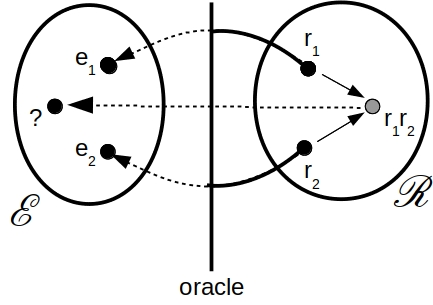
\includegraphics[scale=0.5]{new_topics}
\caption{\label{fig:intro_new_topics}Discovering new research entities.}
\end{figure}

In this book, we explore an alternative strategy for identifying new research directions by combining concepts that are already known. The basic idea is straightforward: by taking two distinct representations, each corresponding to a different known entity, we identify a new entity by joining them into a single representation. To make this approach systematic, we assume that the space of valid representations is closed under such combinations—in other words, that combining any two representations will always yield another valid one. This assumption enables us to construct joint topics in a mechanical way and to explore their potential to uncover novel insights or previously unexamined questions. In practical terms, this involves computing all possible combinations of known entities and selecting those that appear to have the greatest potential to yield new and interesting research directions. However, the precise meaning and significance of any new entity formed in this way must still be determined through further investigation and reflection.

\begin{example}
We could combine compelling topics from the field of theoretical computer science with those from phenomenology to identify promising new research directions. By merging the concepts of "minimum complexity computer programs" and "self-awareness," we arrive at a potential new research topic: "minimum complexity self-aware computers." This would involve investigating the minimum complexity required for a computer program to possess the capacity for self-awareness.
\end{example}


\begin{figure}[h]
\centering
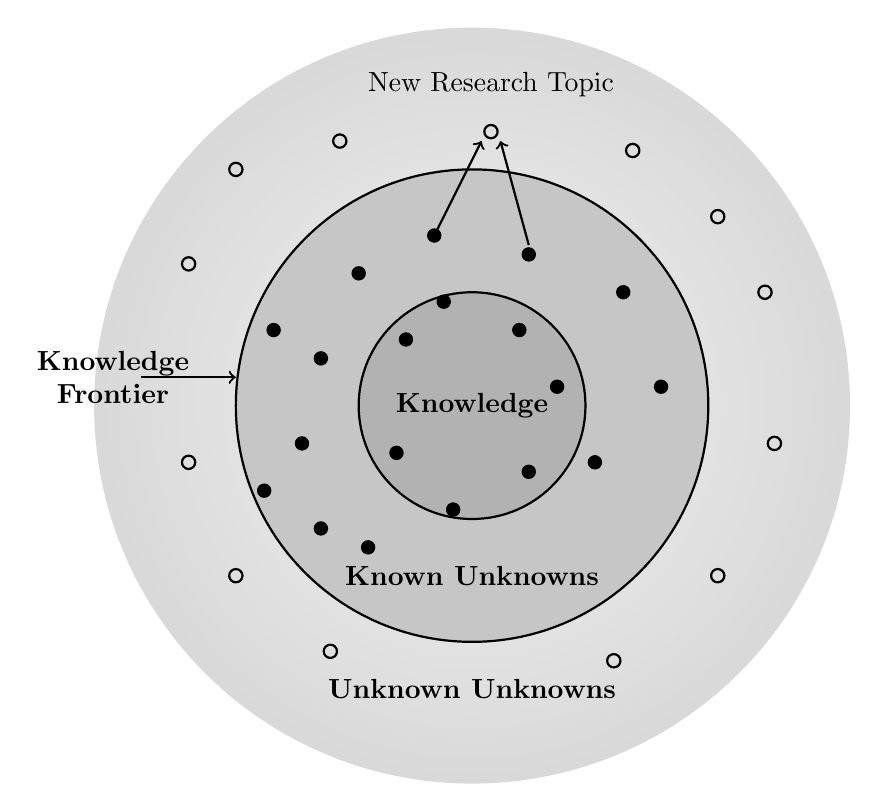
\begin{tikzpicture}[scale=1.2]

% Background gradient only (no border for outermost area)
\shade[inner color=gray!10, outer color=gray!30] (0,0) circle (4);

% Middle circle: Known Unknowns (with border)
\filldraw[fill=gray!45, draw=black, thick] (0,0) circle (2.5);
\node at (0,-3.0) {\textbf{Unknown Unknowns}};
\node at (0,-1.8) {\textbf{Known Unknowns}};

% Inner circle: Knowledge (with border)
\filldraw[fill=gray!60, draw=black, thick] (0,0) circle (1.2);
\node at (0,0) {\textbf{Knowledge}};

% Knowledge Frontier label
\node[align=center] at (-3.8,0.3) {\textbf{Knowledge} \\ \textbf{Frontier}};
\draw[->, thick] (-3.5,0.3) -- (-2.5,0.3);

% Known topics (solid dots)
\foreach \x/\y in {
  -0.7/0.7, -0.3/1.1, 0.5/0.8, 0.9/0.2, 0.6/-0.7, -0.2/-1.1, -0.8/-0.5,
  -1.6/0.5, -1.2/1.4, -0.4/1.8, 0.6/1.6, 1.6/1.2, 2/0.2, 1.3/-0.6,
  -1.1/-1.5, -1.8/-0.4, -2.1/0.8, -2.2/-0.9, -1.6/-1.3
}{
  \filldraw[black] (\x,\y) circle (2pt);
}

% Unknown unknowns (hollow circles)
\foreach \x/\y in {
  -3/1.5, -2.5/2.5, -1.4/2.8, 0.2/2.9, 1.7/2.7, 2.6/2, 3.1/1.2,
  3.2/-0.4, 2.6/-1.8, 1.5/-2.7, -1.5/-2.6, -2.5/-1.8, -3/-0.6
}{
  \draw[black, thick] (\x,\y) circle (2pt);
}

% Arrows pointing to new topics
\draw[->, thick] (-0.4,1.8) -- (0.1,2.8);
\draw[->, thick] (0.6,1.7) -- (0.3,2.8);
\node at (0.2,3.4) {\text{New Research Topic}};

\end{tikzpicture}
\caption{\label{fig:NewTopics}The structure of knowledge}
\end{figure}

% \begin{figure}[h]
% \centering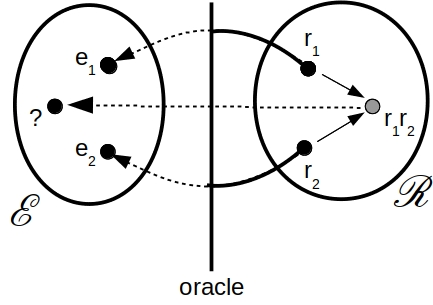
\includegraphics[scale=0.5]{new_topics}
% \caption{\label{fig:intro_new_topics}Discovering new research entities.}
% \end{figure}

% \begin{figure}[h]
% \centering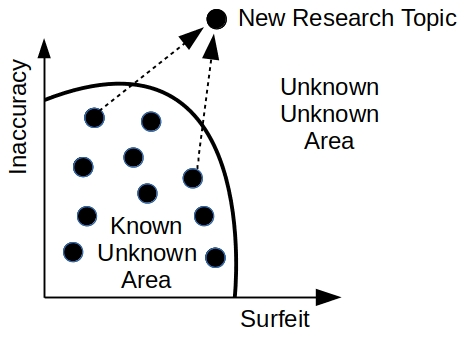
\includegraphics[scale=0.5]{NewTopics}
% \caption{\label{fig:NewTopics}New Research Topics}
% \end{figure}

As wisely stated by Saint John of the Cross, \emph{to go where we do not know, we must go by a path we do not know}. This insight holds true in scientific discovery: the likelihood that a combination of two already known entities leads to a new entity located in the unknown unknown is greater when the entities being combined are themselves poorly understood. In contrast, combining well-understood entities is more likely to produce a result that remains within the bounds of current knowledge—that is, inside the knowledge frontier (see Figure \ref{fig:NewTopics}). This is because the areas surrounding a well-known entity are often already thoroughly explored, leaving little room for the kind of novelty we are looking for, namely, ideas that lie beyond the current boundaries of knowledge and have the potential to open up entirely new lines of inquiry.

Another approach to increasing the chances of reaching the unknown unknown is by combining topics from two distinct fields of knowledge. The likelihood that such a combination has already been explored is relatively low, primarily because it would require someone with substantial expertise in both areas—a rarity in today's academic landscape, where scientists are increasingly specialized in narrow domains. Interdisciplinary combinations, therefore, offer a fertile ground for novel discoveries, as they may produce connections that have never been examined or even imagined within the confines of a single discipline.

%
% Section: References
%

\section*{References}

The theory of nescience builds upon several well-established foundations across information theory, computability, algorithmic complexity, and the philosophy of science. The following references provide the theoretical background and conceptual tools necessary to understand and contextualize the ideas introduced in this chapter.
 
Sipser's book \cite{sipser2012introduction} is a widely respected introduction to formal languages, automata, and computability theory. It lays the groundwork for understanding which descriptions are computationally feasible, an essential aspect of the theory of nescience, which assumes that knowledge must be computable to be meaningful.

\cite{li2013introduction} is a comprehensive volume that presents the theory of Kolmogorov complexity, which formalizes the idea of description length using the shortest program capable of generating a given object. The concepts developed by Li and Vitányi are central to the theory of nescience, especially in defining metrics such as inaccuracy, miscoding, and surfeit based on algorithmic information.

Chalmers' book \cite{chalmers2013thing} offers a critical and historical introduction to the philosophy of science. It examines the assumptions, limits, and methodologies of scientific practice. This perspective is invaluable for situating the theory of nescience within the broader discourse on how scientific knowledge is constructed, evaluated, and refined over time.

\cite{cover2012elements} is a foundational text in information theory, providing the mathematical framework for understanding concepts such as entropy, mutual information, and data compression. It serves as a rigorous yet accessible introduction to how information can be quantified, transmitted, and encoded, ideas that relate the notions of description length in the theory of nescience.